\documentclass[conference]{IEEEtran}
\usepackage[T1]{fontenc}
\usepackage{graphicx}
\usepackage{booktabs}
\usepackage{array}
\newcolumntype{L}[1]{>{\raggedright\arraybackslash}p{#1}}
\usepackage{microtype}
\usepackage{url}
\usepackage[hidelinks]{hyperref}

\newcommand{\K}{$K$}

\begin{document}

\title{Memory-Aware Agent Edge Serving\\
\large Phase 1: Baseline and Bottleneck Characterization}

\author{\IEEEauthorblockN{Jiawei Liu, Kaiqi Han, Tianyu Xu, You Chen, Yufan Shi}
\IEEEauthorblockA{University of California San Diego \quad CSE 291A, Fall 2026}}

\maketitle

\begin{abstract}
We characterize what limits completed work when tool-using agents share one GPU under a bounded KV
budget. Across 29 runs (5,890 tasks) of HotpotQA ReAct agents on llama.cpp, we find two regimes. With
ample memory, throughput peaks at 8 concurrent agents and then declines, because attention cost in the
unified KV pool grows with all resident tokens. Under a tight budget, over-commitment fails every
in-flight request and contexts grow 2--4$\times$ per task, so safe concurrency falls far below the
compute optimum while a quarter of the pool is held by agents waiting on tools.
\end{abstract}

\section{Introduction}

Agent tasks issue several dependent requests whose context grows with every step, and between requests
the agent waits on a tool while its KV cache remains resident. On a memory-constrained device, admitting
too many agents exhausts the KV budget; admitting too few leaves the accelerator idle.

We study this trade-off on a single GPU serving ReAct agents~\cite{react} with a local 7B
model~\cite{qwen} through llama.cpp~\cite{llamacpp}. Phase~1 asks which resource limits completed work
under a bounded KV budget: (a) KV capacity for active requests, (b) KV held by agents idle in tool calls,
(c) re-prefill after the runtime evicts a context, or (d) the GPU itself when memory never binds. We
contribute a reproducible, instrumented workload, a FIFO fixed-concurrency baseline, and measurements
that separate these effects.

\section{Workload and Methodology}

\subsection{Workload}
Agents answer HotpotQA multi-hop questions~\cite{hotpotqa}, searching an offline corpus of 66,581
paragraphs. HotpotQA annotates supporting facts, so every retrieved sentence in a context can be labeled
as evidence or not, which measures how much KV is useful rather than only how much is used. The prompt
grows append-only, so each step's prompt is a prefix of the next. Four profiles cover the required mix:
\texttt{react\_short} (contexts near 2k tokens), \texttt{react\_long} (growing from 1.5k to 3--7k),
\texttt{react\_explain} (300 extra output tokens), and \texttt{oneshot\_long} (one 3.3k-token request).
Tool latency is lognormal (median 0.8\,s) and seeded per task, step, and tool, so all configurations
replay identical delays. Frozen workloads with closed-loop or Poisson arrivals are drawn from a
1,500-question split. The agent reaches an F1 of 0.64, versus 0.25 closed-book.

\subsection{Baseline and Measurement}
We serve Qwen2.5-7B-Instruct (Q4\_K\_M, f16 KV) with \texttt{llama-server} b11960 on an NVIDIA A10G;
the KV budget is the unified pool shared by all slots (\texttt{-c}). The baseline admits tasks in FIFO
order to \K{} workers, and worker $k$ pins slot $k$, so an agent's KV stays resident through its tool
calls. We record per-request tokens and timings, tool waits, and per-task latency, queueing, and EM/F1,
and reconstruct per-slot KV occupancy, attributed to agents in a request, idle in a tool call, or
finished. Throughput is measured between the 10th and 90th percentile completion. Runtime probes and
microbenchmarks cover overflow, eviction, prefill, decode, and offload costs. F1 stays within
0.52--0.64 in every configuration that completes at least 85\% of its tasks.

\begin{figure*}[t]
  \centering
  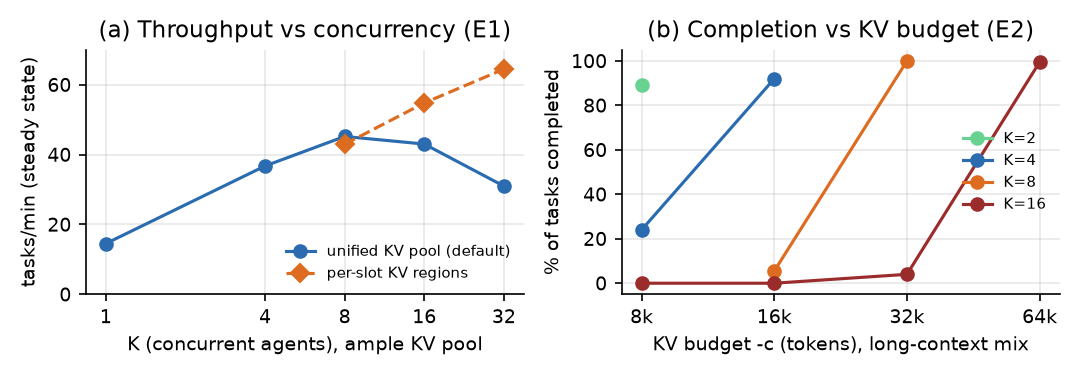
\includegraphics[width=0.8\textwidth]{../figures/phase1/summary.png}
  \caption{(a) Steady-state throughput versus concurrency \K{} with an ample KV pool (131k tokens), for
  llama.cpp's unified pool and for per-slot KV regions. (b) Fraction of tasks completed as the KV budget
  shrinks, long-context mix (70\% \texttt{react\_long}).}
  \label{fig:summary}
\end{figure*}

\section{Results}

\begin{table}[t]
  \caption{Summary of Phase 1 Experiments}
  \label{tab:results}
  \centering
  \footnotesize
  \setlength{\tabcolsep}{3pt}
  \begin{tabular}{@{}L{0.19\columnwidth}L{0.31\columnwidth}L{0.46\columnwidth}@{}}
    \toprule
    Experiment & Setting & Result \\
    \midrule
    Concurrency & \K{} = 1/4/8/16/32 & 14.5/36.8/\textbf{45.2}/43.0/31.0 tasks/min \\
    Per-slot KV & \K{} = 8/16/32 & 43.0/\textbf{54.8}/\textbf{64.5} tasks/min \\
    Open loop & \K{} = 8; 21/33/45 arr./min & p95 latency 16.5/21.1/30.7\,s \\
    KV budget & 8k/16k/32k/64k tokens & max.\ working \K{} = 2/4/8/16; 22.8/37.8/47.8/47.3 tasks/min \\
    Tool delay & $\times$0/1/4, \K{} = 16 & 44.1/43.0/41.0 tasks/min; idle KV 0/8/33\% \\
    Prefix reuse & \K{} = 8 & no reuse: 36\% of baseline; runtime slot choice: $-$17\% \\
    \bottomrule
  \end{tabular}
\end{table}

Table~\ref{tab:results} summarizes the experiments and Fig.~\ref{fig:summary} shows the two central
results.

\subsection{Concurrency and the Unified KV Pool}
With an ample pool, throughput peaks at $K=8$ and falls by 31\% at $K=32$, although the work per task is
constant. The median time per generated token rises from 15\,ms at $K=4$ to 254\,ms at $K=32$, against
28\,ms for 32 decodes with separate KV buffers. In the unified pool, attention cost appears to scale with
the tokens of all slots: at batch 16, prefill drops from 4,578 to 2,776\,tok/s when requests share the
pool. A fixed KV region per slot removes most of the decline (+27\% at $K=16$ with the same 131k-token
budget, 2.1$\times$ at $K=32$ with twice the pool), at the cost of static reservation.

\subsection{KV Budget and Context Growth}
When the active working set exceeds the pool, the runtime fails every in-flight request instead of
queueing, and the workers' next tasks fail likewise. Doubling \K{} beyond the budget reduces completion
from 89--100\% to at most 24\% (Fig.~\ref{fig:summary}b); 971 of 972 failures are context overflows.
Context growth forces conservative provisioning: a \texttt{react\_long} agent grows from a median of
1,488 tokens to a median peak of 3,437 and a 95th-percentile peak of 6,226. The largest working \K{} is
about the budget divided by 4k tokens, and 8k and 16k budgets reach only 48\% and 80\% of the throughput
of larger ones.

\subsection{Idle KV and Tool Latency}
With an ample pool, scaling tool delays by four leaves 33\% of the held KV idle but costs only 7\% of
throughput, since other agents keep the GPU busy. At the small \K{} that tight budgets impose, 36--44\% of
the held KV (about a quarter of the pool) belongs to agents waiting on tools; this share depends on \K{},
not on memory pressure.

\subsection{Retained Context and Runtime Policy}
Disabling prefix reuse increases prefill work 4.9$\times$ and cuts throughput to 36\%. When llama.cpp
assigns slots itself, 31\% of returning steps land on another slot and re-prefill, costing 17\%. Under
pressure it evicts the idle slot with the lowest index, regardless of recency or size. Offloading 2k
tokens to host memory takes 113\,ms and stalls all other slots meanwhile; re-prefilling takes 0.45\,s
(2k tokens) to 1.97\,s (8k).

\subsection{KV Composition}
The 1.4k-token ReAct prefix accounts for 73\% of a \texttt{react\_short} context and is stored separately
in every slot. In \texttt{react\_long} contexts only 4.5\% of retrieved tokens are supporting facts.

\section{Dominant Bottleneck}
With ample memory, throughput is limited by attention cost in the unified pool (d), which caps useful
concurrency at $K\approx8$ on this GPU. Under a tight budget, active KV capacity (a) binds: contexts grow
and overflow fails all in-flight work, so a fixed \K{} must be provisioned for peak demand and the GPU is
underutilized. Idle KV (b) is a large share of the pool only in this regime. Re-prefill after eviction
(c) was rare under the always-retain baseline (at most 12 live-agent evictions per run) but costly.

\section{Phase 2 Plan}
Phase~2 targets the memory-constrained regime with one mechanism: an agent-level KV lifecycle manager at
tool-call boundaries, combined with admission that reserves each agent's projected peak KV. Unlike
InferCept~\cite{infercept}, built on vLLM~\cite{vllm}, it must use llama.cpp's slot save, restore, and
erase controls, whose offload path blocks all slots. Because releasing KV costs more than retaining it
through a typical tool call (break-even 1.7--3.0\,s at $K=16$ versus a 0.8\,s median delay), the policy
retains by default and releases the agent expected to return last only under pressure. Baselines are the
best fixed \K{} per budget, per-slot KV regions, and the runtime's default policy, evaluated across
arrival rates, mixes, and low-benefit cases.

\begin{thebibliography}{6}
\footnotesize
\bibitem{hotpotqa} Z.~Yang \emph{et al.}, ``HotpotQA: A dataset for diverse, explainable multi-hop question
answering,'' in \emph{Proc. EMNLP}, 2018.
\bibitem{react} S.~Yao \emph{et al.}, ``ReAct: Synergizing reasoning and acting in language models,'' in
\emph{Proc. ICLR}, 2023.
\bibitem{llamacpp} G.~Gerganov \emph{et al.}, ``llama.cpp,'' \url{https://github.com/ggml-org/llama.cpp}.
\bibitem{qwen} Qwen Team, ``Qwen2.5 technical report,'' arXiv:2412.15115, 2024.
\bibitem{infercept} R.~Abhyankar \emph{et al.}, ``InferCept: Efficient intercept support for augmented
large language model inference,'' in \emph{Proc. ICML}, 2024.
\bibitem{vllm} W.~Kwon \emph{et al.}, ``Efficient memory management for large language model serving
with PagedAttention,'' in \emph{Proc. SOSP}, 2023.
\end{thebibliography}

\onecolumn
\appendix[Timeline and Milestones]
\vspace{4pt}

\begin{center}
  \small
  \setlength{\tabcolsep}{5pt}
  \begin{tabular}{@{}L{0.11\textwidth}L{0.5\textwidth}L{0.24\textwidth}L{0.08\textwidth}@{}}
    \toprule
    Dates & Work & Milestone & Status \\
    \midrule
    10/21--10/28 & Design; data, corpus, splits; tools, ReAct agent, profiles; workload generator; FIFO
      runner and instrumentation & End-to-end workload on 7B & Done \\
    10/29--10/31 & AWS A10G setup; cost model; runtime probes; microbenchmarks; experiments E1--E5 &
      Measurements and bottleneck analysis & Done \\
    11/1--11/4 & Phase 1 report & \textbf{Phase 1 due 11/4} & Done \\
    11/5--11/11 & KV manager (slot save/restore/erase); peak-KV admission; baselines including per-slot
      KV & All baselines run end to end & Planned \\
    11/12--11/18 & Pressure-gated retention policy; tuning on dev; idle-KV cost test & Main comparison
      on dev & Planned \\
    11/19--12/2 & Arrival-rate, mix and no-benefit sweeps on test; admission and lifecycle ablation;
      overhead and fairness & All Phase 2 results & Planned \\
    12/3--12/9 & Final report and reproducibility package & \textbf{Final submission} & Planned \\
    \bottomrule
  \end{tabular}
\end{center}

\end{document}
